\begin{figure*}[h!t!]
  \caption{High Level Architecture}
  \centering
    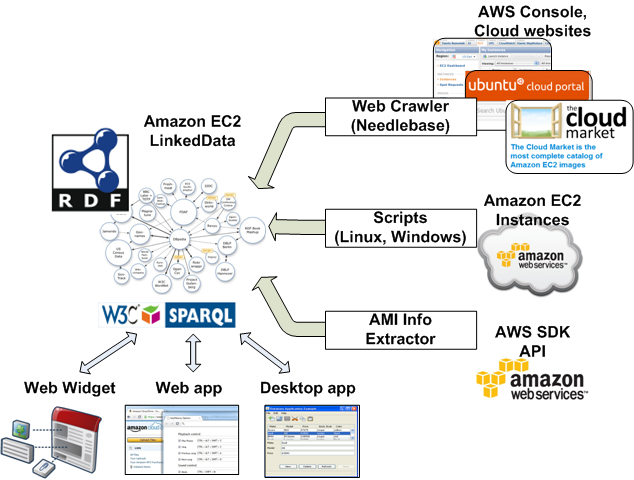
\includegraphics[width=0.5\textwidth]{EC2LD.png}
   \label{fig:architecture}
\end{figure*}

\section{Amazon EC2 AMI}\label{sec:ec2}

Nowadays the advancements of cloud computing have made it possible for us to have different environments for computing without having the need to have a dedicated infrastructure for each of the different environments we require. One of the main advantage of virtualized environment is that it is possible to recreate the same environment as many times as you want with a minimal effort. This put the computer users lives at ease because they can use a virtual machines for different temporary tasks without having the trouble to change the configuration of the personal machines. This ability can be very useful in scenarios like reproducing environments for software testing, to try out software before installing them on a physical machine i.e. as a staging machine. 

If it is possible to use already prepared virtual machines which matches the requirements, for example, the architecture, i.e., it is 32 bits or 64 bits, the operation system, storage and memory requirements it would save a lot of time and effort of people trying to prepare a computing environment for a given task. In other words, if we could facilitate the search and discovery of virtual machine images in a systematic way, we could build a lot of semantic applications on top of this that will automate this process and make the use of cloud computing for these tasks much easier. 


\section{Amazon EC2 Linked Data Life Cycle}\label{sec:process}
In this section we briefly describe our process for generating, interconnecting, and publishing EC2 AMI linked data. This process was inspired by existing methodological guidelines \cite{VillazonTerrazas_2011}, which propose an iterative incremental life cycle model where EC2 AMI LD gets
continuously improved and extended. Our goal of this project is to create a LinkedData dataset about Amazon virtual machine images. Thanks to this dataset, we have been able to build applications which can query the dataset using the defined ontology and help the users find Amazon Machine Images (AMI) that suit their requirements. Figure \ref{fig:architecture} shows the high level architecture.

\subsection{Use cases for AmazonMachineImage reuse}
Among many other advantages of cloud computing like scalability, high accessibility, and cost saving the ability to reuse a virtual machine as many times becomes a time saver in most of the cloud scenarios. Most cloud users create several master templates of the virtual machines images and use the appropriate one whenever necessary. This is far more efficient compared to setting up physical machines as the virtual machine images which are not currently executing will only consume storage space but no CPU power or memory. It is even better if one can use a public virtual machine image which satisfies the task at hand because it bring the setting up time to a bare minimum. 

There are many use cases where it is very useful to find and reuse an existing virtual machine image without spending time on preparing the environment. For example, one might want to find a virtual machine environment which has a similar characteristics to a physical machine to experiment different configurations or settings without having the risk of corrupting the own machines. It also make it possible to start things from the scratch with another instance of the same virtual image. Moreover, it is becoming common for software vendors to provide links to public virtual machine images which the users can use as a sandbox to first try the software on a virtual machine without installing on their own machines.    

\subsection{Amazon Machine Image data extraction}
Amazon EC2 LinkedData dataset is created by merging the data acquired by several different sources. The main source is the API provided by AWS SDK for Java \footnote{\url{http://aws.amazon.com/documentation/sdkforjava/}}. An AMI Information Extractor java application will iterate through all the public Amazon Virtual Machine images and extract the data available from the API. However, the AWS SDK lacks the ability to extract several important attributes like operating system, or the image size which are essential to make this dataset useful in real life scenarios. The challenge is overcome by extracting information from other sources and aggregating them to the dataset. There are websites and portals which provides a richer set of attributes about Amazon Machine Images which contains the aforementioned information as unstructured data available as wep pages. Examples of these sites include the AWS Management Console \footnote{http://aws.amazon.com/console/}, Ubuntu Cloud Portal \footnote{http://cloud.ubuntu.com/}, and The Cloud Market catalog {http://thecloudmarket.com/}. Needlebase platform \footnote{http://needlebase.com/} is used to acquiring, integrating, and cleansing information from these sites and feed them to the Amazon EC2 LinkedData dataset. Even more detailed information about a given AMI can be extracted by a running scripts inside the Amazon instances created using the given AMI. Two scripts for Windows and Linux are made available for Amazon users which they can run to upload additional data about an AMI.       

Finally, it is worth mentioning that the SPARL endpoint is available at \url{http://mccarthy.dia.fi.upm.es:8892/sparql}.
\vspace{5mm}
\section{EC2LD applications}\label{sec:apps}
We have built three applications which consumes the Amazon EC2 LinkedData and provide users AmazonMachineImage ids which match their requirements. These applications are a web widget, a desktop application, a web application. The web widget which is implemented as a Google Gadget \footnote{https://developers.google.com/gadgets/} can be embedded in web pages. Once configured with certain properties, this widget can communicate with the SPARQL endpoint and dynamically fetch the amazon virtual machine images which match the requirements. Figure \ref{fig:config} shows an example of the parameters. This can be a good addition to the software providers i.e. they can include this widget in the download pages so that users know in which public virtual machine images they can try this software.

\begin{figure}[h!t!]
  \caption{Configuration parameters of the web widget}
  \centering
    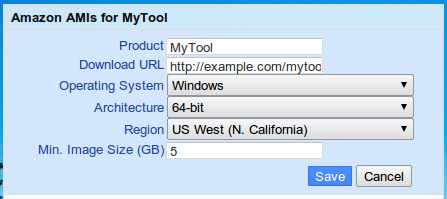
\includegraphics[width=0.5\textwidth]{gadget-config.png}
   \label{fig:config}
\end{figure}



The VMI Finder desktop application can run on a computing environment and gather the data and then will create a SPARQL query based on those information to query the SPARQL endpoint exposed by Amazon EC2 LinkedData. Users can manually modify the information that has been automatically collected before executing the query by editing, adding, or removing any information. The query result will provide a set of AmazonMachineImage ids which matches the computing environment it runs. The web application also provide a similar functionality where users can directly search for AmazonMachineImages via a web interface. Figure \ref{fig:results} depicts the search results.

\begin{figure}[h!t!]
  \caption{Search results of the web widget}
  \centering
    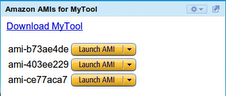
\includegraphics[scale=0.8]{gadget-results.png}
   \label{fig:results}
\end{figure}

The applications are available at \url{http://mccarthy.dia.fi.upm.es/ec2ld/}